\documentclass[a4paper,11pt]{article}
\usepackage[utf8]{inputenc}\usepackage[T1]{fontenc}
\usepackage[english]{babel}\usepackage{lmodern}\usepackage{microtype}
\usepackage{amsmath,amssymb}\usepackage{geometry}
\geometry{a4paper,left=2.2cm,right=2.2cm,top=2.0cm,bottom=2.0cm}
\usepackage{booktabs,array}\usepackage{xcolor}
\definecolor{bokug}{RGB}{0,135,60}\usepackage{tikz}
\usetikzlibrary{arrows.meta,calc}
\usepackage{fancyhdr}\pagestyle{fancy}
\renewcommand{\headrulewidth}{0.4pt}
\usepackage{enumitem}\setlength{\parindent}{0pt}\setlength{\parskip}{4pt}

\begin{document}
\fancyhead[L]{\small VU Mechanik – LAWI 100515 (PI)}\fancyhead[R]{\small SS 2026}\fancyfoot[C]{\thepage}
\begin{center}{\large\bfseries\color{bokug}University of Natural Resources and Life Sciences, Vienna (BOKU)}\\[2pt]{\large\bfseries VU Mechanik – LAWI 100515 (PI)}\\[4pt]Exam \textbf{Group A} \hfill Date: 26.06.2026\\[2pt]\rule{\linewidth}{0.4pt}\end{center}

\begin{center}\textbf{\large Model solution}\end{center}
\begin{center}
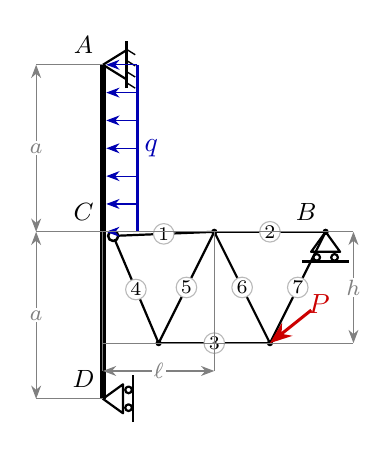
\begin{tikzpicture}[scale=0.707,>=Stealth,line join=round]
  \coordinate (P0) at (0.000,0.000);
  \coordinate (P1) at (0.000,-3.000);
  \coordinate (P2) at (0.000,-6.000);
  \coordinate (TO1) at (2.000,-3.000);
  \coordinate (TO2) at (4.000,-3.000);
  \coordinate (TU0) at (1.000,-5.000);
  \coordinate (TU1) at (3.000,-5.000);
  \coordinate (CPIN) at (0.184,-3.074);
  \draw[thick] (CPIN) -- (TO1);
  \draw[thick] (TO1) -- (TO2);
  \draw[thick] (TU0) -- (TU1);
  \draw[thick] (CPIN) -- (TU0);
  \draw[thick] (TU0) -- (TO1);
  \draw[thick] (TO1) -- (TU1);
  \draw[thick] (TU1) -- (TO2);
  \draw[line width=2.2pt] (P0) -- (P1);
  \draw[line width=2.2pt] (P1) -- (P2);
  \fill (TO1) circle (1.6pt);
  \fill (TO2) circle (1.6pt);
  \fill (TU0) circle (1.6pt);
  \fill (TU1) circle (1.6pt);
  \draw[fill=white,line width=0.9pt] (CPIN) circle (2.6pt);
  \draw[thick] (0.000,0.000) -- (0.420,-0.260) -- (0.420,0.260) -- cycle;
  \draw[line width=1pt] (0.420,-0.420) -- (0.420,0.420);
  \draw[line width=0.5pt] (0.420,-0.320) -- (0.580,-0.420);
  \draw[line width=0.5pt] (0.420,-0.120) -- (0.580,-0.220);
  \draw[line width=0.5pt] (0.420,0.080) -- (0.580,-0.020);
  \draw[line width=0.5pt] (0.420,0.280) -- (0.580,0.180);
  \draw[thick] (0.000,-6.000) -- (0.360,-6.260) -- (0.360,-5.740) -- cycle;
  \draw[thick] (0.460,-6.160) circle (0.06) (0.460,-5.840) circle (0.06);
  \draw[line width=1pt] (0.540,-6.420) -- (0.540,-5.580);
  \draw[thick] (4.000,-3.000) -- (3.740,-3.360) -- (4.260,-3.360) -- cycle;
  \draw[thick] (3.840,-3.460) circle (0.06) (4.160,-3.460) circle (0.06);
  \draw[line width=1pt] (3.580,-3.540) -- (4.420,-3.540);
  \node[circle,fill=white,draw=gray!55,inner sep=0.5pt,font=\scriptsize] at (1.092,-3.037) {1};
  \node[circle,fill=white,draw=gray!55,inner sep=0.5pt,font=\scriptsize] at (3.000,-3.000) {2};
  \node[circle,fill=white,draw=gray!55,inner sep=0.5pt,font=\scriptsize] at (2.000,-5.000) {3};
  \node[circle,fill=white,draw=gray!55,inner sep=0.5pt,font=\scriptsize] at (0.592,-4.037) {4};
  \node[circle,fill=white,draw=gray!55,inner sep=0.5pt,font=\scriptsize] at (1.500,-4.000) {5};
  \node[circle,fill=white,draw=gray!55,inner sep=0.5pt,font=\scriptsize] at (2.500,-4.000) {6};
  \node[circle,fill=white,draw=gray!55,inner sep=0.5pt,font=\scriptsize] at (3.500,-4.000) {7};
  \draw[->,blue!70!black] (0.620,0.000) -- (0.060,0.000);
  \draw[->,blue!70!black] (0.620,-0.500) -- (0.060,-0.500);
  \draw[->,blue!70!black] (0.620,-1.000) -- (0.060,-1.000);
  \draw[->,blue!70!black] (0.620,-1.500) -- (0.060,-1.500);
  \draw[->,blue!70!black] (0.620,-2.000) -- (0.060,-2.000);
  \draw[->,blue!70!black] (0.620,-2.500) -- (0.060,-2.500);
  \draw[->,blue!70!black] (0.620,-3.000) -- (0.060,-3.000);
  \draw[blue!70!black,thick] (0.620,0.000) -- (0.620,-3.000);
  \node[blue!70!black] at (0.870,-1.500) {$q$};
  \draw[->,red!80!black,line width=1.1pt] (3.742,-4.407) -- (3.000,-5.000);
  \node[red!80!black] at (3.882,-4.294) {$P$};
  \draw[thin,gray] (0.000,0.000) -- (-1.200,0.000);
  \draw[thin,gray] (0.000,-3.000) -- (-1.200,-3.000);
  \draw[<->,gray] (-1.200,0.000) -- (-1.200,-3.000) node[midway,fill=white,inner sep=0.8pt,font=\footnotesize]{$a$};
  \draw[thin,gray] (0.000,-3.000) -- (-1.200,-3.000);
  \draw[thin,gray] (0.000,-6.000) -- (-1.200,-6.000);
  \draw[<->,gray] (-1.200,-3.000) -- (-1.200,-6.000) node[midway,fill=white,inner sep=0.8pt,font=\footnotesize]{$a$};
  \draw[thin,gray] (0.000,-3.000) -- (0.000,-5.500);
  \draw[thin,gray] (2.000,-3.000) -- (2.000,-5.500);
  \draw[<->,gray] (0.000,-5.500) -- (2.000,-5.500) node[midway,fill=white,inner sep=0.8pt,font=\footnotesize]{$\ell$};
  \draw[thin,gray] (0.000,-3.000) -- (4.500,-3.000);
  \draw[thin,gray] (0.000,-5.000) -- (4.500,-5.000);
  \draw[<->,gray] (4.500,-3.000) -- (4.500,-5.000) node[midway,fill=white,inner sep=0.8pt,font=\footnotesize]{$h$};
  \node[font=\small] at (0.000,0.000) [xshift=-7pt,yshift=7pt] {$A$};
  \node[font=\small] at (0.000,-3.000) [xshift=-7pt,yshift=7pt] {$C$};
  \node[font=\small] at (0.000,-6.000) [xshift=-7pt,yshift=7pt] {$D$};
  \node[font=\small] at (4.000,-3.000) [xshift=-7pt,yshift=7pt] {$B$};
\end{tikzpicture}
\end{center}
\par\medskip\textbf{1.\ Static determinacy}\par Counting criterion $n=3k-(a+z)$ (bodies $k$, reactions $a$, interaction forces $z$):
\[ n=3k-(a+z)=3\cdot2-(4+2)=0\ \Rightarrow\ \text{statically determinate} \]
\par\medskip\textbf{2.\ Support reactions and hinge forces}\par
$A:\ R_x=14,\ R_y=-3$\quad $D:\ R_x=8,\ R_y=0$\quad $B:\ R_x=0,\ R_y=11$\par $C:\ H_x=-10,\ H_y=3$
\par\medskip\textbf{3.\ Truss member forces}\par
\begin{center}\renewcommand{\arraystretch}{1.1}\begin{tabular}{c r l}
\toprule
Member & Force $S$ [kN] & Type \\
\midrule
  1 & -8.5 & compression \\
  2 & -5.5 & compression \\
  3 & -3 & compression \\
  4 & -3.35 & compression \\
  5 & 3.35 & tension \\
  6 & -3.35 & compression \\
  7 & 12.3 & tension \\
\bottomrule
\end{tabular}\end{center}
\begin{center}
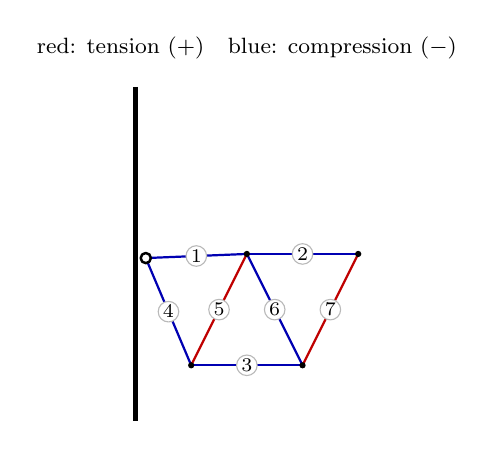
\begin{tikzpicture}[scale=0.707,>=Stealth,line join=round]
  \coordinate (P0) at (0.000,0.000);
  \coordinate (P1) at (0.000,-3.000);
  \coordinate (P2) at (0.000,-6.000);
  \coordinate (TO1) at (2.000,-3.000);
  \coordinate (TO2) at (4.000,-3.000);
  \coordinate (TU0) at (1.000,-5.000);
  \coordinate (TU1) at (3.000,-5.000);
  \coordinate (CPIN) at (0.184,-3.074);
  \draw[thick,blue!70!black] (CPIN) -- (TO1);
  \draw[thick,blue!70!black] (TO1) -- (TO2);
  \draw[thick,blue!70!black] (TU0) -- (TU1);
  \draw[thick,blue!70!black] (CPIN) -- (TU0);
  \draw[thick,red!75!black] (TU0) -- (TO1);
  \draw[thick,blue!70!black] (TO1) -- (TU1);
  \draw[thick,red!75!black] (TU1) -- (TO2);
  \draw[line width=2pt] (P0) -- (P1);
  \draw[line width=2pt] (P1) -- (P2);
  \fill (TO1) circle (1.6pt);
  \fill (TO2) circle (1.6pt);
  \fill (TU0) circle (1.6pt);
  \fill (TU1) circle (1.6pt);
  \draw[fill=white,line width=0.9pt] (CPIN) circle (2.6pt);
  \node[circle,fill=white,draw=gray!55,inner sep=0.5pt,font=\scriptsize] at (1.092,-3.037) {1};
  \node[circle,fill=white,draw=gray!55,inner sep=0.5pt,font=\scriptsize] at (3.000,-3.000) {2};
  \node[circle,fill=white,draw=gray!55,inner sep=0.5pt,font=\scriptsize] at (2.000,-5.000) {3};
  \node[circle,fill=white,draw=gray!55,inner sep=0.5pt,font=\scriptsize] at (0.592,-4.037) {4};
  \node[circle,fill=white,draw=gray!55,inner sep=0.5pt,font=\scriptsize] at (1.500,-4.000) {5};
  \node[circle,fill=white,draw=gray!55,inner sep=0.5pt,font=\scriptsize] at (2.500,-4.000) {6};
  \node[circle,fill=white,draw=gray!55,inner sep=0.5pt,font=\scriptsize] at (3.500,-4.000) {7};
  \node[font=\footnotesize] at (2.00,0.70) {red: tension $(+)$\quad blue: compression $(-)$};
\end{tikzpicture}
\end{center}
\par\medskip\textbf{4.\ Section-force diagrams of the beams}\par
\begin{center}
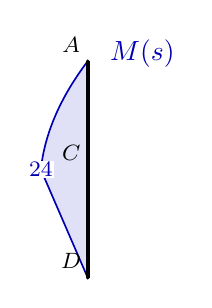
\begin{tikzpicture}[scale=0.459,line join=round]
  \filldraw[fill=blue!70!black!12,draw=blue!70!black,semithick] (0.000,0.000) -- (-0.093,-0.125) -- (-0.183,-0.250) -- (-0.269,-0.375) -- (-0.352,-0.500) -- (-0.432,-0.625) -- (-0.508,-0.750) -- (-0.581,-0.875) -- (-0.650,-1.000) -- (-0.716,-1.125) -- (-0.779,-1.250) -- (-0.838,-1.375) -- (-0.894,-1.500) -- (-0.946,-1.625) -- (-0.995,-1.750) -- (-1.041,-1.875) -- (-1.083,-2.000) -- (-1.122,-2.125) -- (-1.158,-2.250) -- (-1.190,-2.375) -- (-1.219,-2.500) -- (-1.244,-2.625) -- (-1.266,-2.750) -- (-1.285,-2.875) -- (-1.300,-3.000) -- (-1.300,-3.000) -- (-1.246,-3.125) -- (-1.192,-3.250) -- (-1.137,-3.375) -- (-1.083,-3.500) -- (-1.029,-3.625) -- (-0.975,-3.750) -- (-0.921,-3.875) -- (-0.867,-4.000) -- (-0.812,-4.125) -- (-0.758,-4.250) -- (-0.704,-4.375) -- (-0.650,-4.500) -- (-0.596,-4.625) -- (-0.542,-4.750) -- (-0.488,-4.875) -- (-0.433,-5.000) -- (-0.379,-5.125) -- (-0.325,-5.250) -- (-0.271,-5.375) -- (-0.217,-5.500) -- (-0.163,-5.625) -- (-0.108,-5.750) -- (-0.054,-5.875) -- (0.000,-6.000) -- (0.000,-6.000) -- (0.000,-5.875) -- (0.000,-5.750) -- (0.000,-5.625) -- (0.000,-5.500) -- (0.000,-5.375) -- (0.000,-5.250) -- (0.000,-5.125) -- (0.000,-5.000) -- (0.000,-4.875) -- (0.000,-4.750) -- (0.000,-4.625) -- (0.000,-4.500) -- (0.000,-4.375) -- (0.000,-4.250) -- (0.000,-4.125) -- (0.000,-4.000) -- (0.000,-3.875) -- (0.000,-3.750) -- (0.000,-3.625) -- (0.000,-3.500) -- (0.000,-3.375) -- (0.000,-3.250) -- (0.000,-3.125) -- (0.000,-3.000) -- (0.000,-3.000) -- (0.000,-2.875) -- (0.000,-2.750) -- (0.000,-2.625) -- (0.000,-2.500) -- (0.000,-2.375) -- (0.000,-2.250) -- (0.000,-2.125) -- (0.000,-2.000) -- (0.000,-1.875) -- (0.000,-1.750) -- (0.000,-1.625) -- (0.000,-1.500) -- (0.000,-1.375) -- (0.000,-1.250) -- (0.000,-1.125) -- (0.000,-1.000) -- (0.000,-0.875) -- (0.000,-0.750) -- (0.000,-0.625) -- (0.000,-0.500) -- (0.000,-0.375) -- (0.000,-0.250) -- (0.000,-0.125) -- (0.000,0.000) -- cycle;
  \draw[line width=1.6pt] (0.000,0.000) -- (0.000,-3.000) -- (0.000,-6.000);
  \node[blue!70!black,font=\footnotesize,fill=white,inner sep=0.5pt] at (-1.300,-3.000) {24};
  \fill (0.000,0.000) circle (1.3pt);
  \node[font=\footnotesize] at (0.000,0.000) [xshift=-6pt,yshift=6pt] {$A$};
  \fill (0.000,-3.000) circle (1.3pt);
  \node[font=\footnotesize] at (0.000,-3.000) [xshift=-6pt,yshift=6pt] {$C$};
  \fill (0.000,-6.000) circle (1.3pt);
  \node[font=\footnotesize] at (0.000,-6.000) [xshift=-6pt,yshift=6pt] {$D$};
  \node[blue!70!black,right] at (0.35,0.20) {$M(s)$};
\end{tikzpicture}\\[5pt]
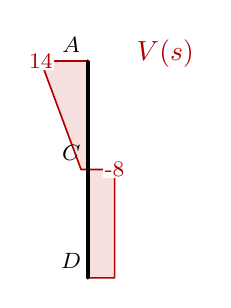
\begin{tikzpicture}[scale=0.459,line join=round]
  \filldraw[fill=red!70!black!12,draw=red!70!black,semithick] (-1.300,0.000) -- (-1.254,-0.125) -- (-1.207,-0.250) -- (-1.161,-0.375) -- (-1.114,-0.500) -- (-1.068,-0.625) -- (-1.021,-0.750) -- (-0.975,-0.875) -- (-0.929,-1.000) -- (-0.882,-1.125) -- (-0.836,-1.250) -- (-0.789,-1.375) -- (-0.743,-1.500) -- (-0.696,-1.625) -- (-0.650,-1.750) -- (-0.604,-1.875) -- (-0.557,-2.000) -- (-0.511,-2.125) -- (-0.464,-2.250) -- (-0.418,-2.375) -- (-0.371,-2.500) -- (-0.325,-2.625) -- (-0.279,-2.750) -- (-0.232,-2.875) -- (-0.186,-3.000) -- (0.743,-3.000) -- (0.743,-3.125) -- (0.743,-3.250) -- (0.743,-3.375) -- (0.743,-3.500) -- (0.743,-3.625) -- (0.743,-3.750) -- (0.743,-3.875) -- (0.743,-4.000) -- (0.743,-4.125) -- (0.743,-4.250) -- (0.743,-4.375) -- (0.743,-4.500) -- (0.743,-4.625) -- (0.743,-4.750) -- (0.743,-4.875) -- (0.743,-5.000) -- (0.743,-5.125) -- (0.743,-5.250) -- (0.743,-5.375) -- (0.743,-5.500) -- (0.743,-5.625) -- (0.743,-5.750) -- (0.743,-5.875) -- (0.743,-6.000) -- (0.000,-6.000) -- (0.000,-5.875) -- (0.000,-5.750) -- (0.000,-5.625) -- (0.000,-5.500) -- (0.000,-5.375) -- (0.000,-5.250) -- (0.000,-5.125) -- (0.000,-5.000) -- (0.000,-4.875) -- (0.000,-4.750) -- (0.000,-4.625) -- (0.000,-4.500) -- (0.000,-4.375) -- (0.000,-4.250) -- (0.000,-4.125) -- (0.000,-4.000) -- (0.000,-3.875) -- (0.000,-3.750) -- (0.000,-3.625) -- (0.000,-3.500) -- (0.000,-3.375) -- (0.000,-3.250) -- (0.000,-3.125) -- (0.000,-3.000) -- (0.000,-3.000) -- (0.000,-2.875) -- (0.000,-2.750) -- (0.000,-2.625) -- (0.000,-2.500) -- (0.000,-2.375) -- (0.000,-2.250) -- (0.000,-2.125) -- (0.000,-2.000) -- (0.000,-1.875) -- (0.000,-1.750) -- (0.000,-1.625) -- (0.000,-1.500) -- (0.000,-1.375) -- (0.000,-1.250) -- (0.000,-1.125) -- (0.000,-1.000) -- (0.000,-0.875) -- (0.000,-0.750) -- (0.000,-0.625) -- (0.000,-0.500) -- (0.000,-0.375) -- (0.000,-0.250) -- (0.000,-0.125) -- (0.000,0.000) -- cycle;
  \draw[line width=1.6pt] (0.000,0.000) -- (0.000,-3.000) -- (0.000,-6.000);
  \node[red!70!black,font=\footnotesize,fill=white,inner sep=0.5pt] at (-1.300,0.000) {14};
  \node[red!70!black,font=\footnotesize,fill=white,inner sep=0.5pt] at (0.743,-3.000) {-8};
  \fill (0.000,0.000) circle (1.3pt);
  \node[font=\footnotesize] at (0.000,0.000) [xshift=-6pt,yshift=6pt] {$A$};
  \fill (0.000,-3.000) circle (1.3pt);
  \node[font=\footnotesize] at (0.000,-3.000) [xshift=-6pt,yshift=6pt] {$C$};
  \fill (0.000,-6.000) circle (1.3pt);
  \node[font=\footnotesize] at (0.000,-6.000) [xshift=-6pt,yshift=6pt] {$D$};
  \node[red!70!black,right] at (1.09,0.20) {$V(s)$};
\end{tikzpicture}\\[5pt]
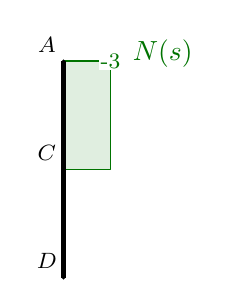
\begin{tikzpicture}[scale=0.459,line join=round]
  \filldraw[fill=green!45!black!12,draw=green!45!black,semithick] (1.300,0.000) -- (1.300,-0.125) -- (1.300,-0.250) -- (1.300,-0.375) -- (1.300,-0.500) -- (1.300,-0.625) -- (1.300,-0.750) -- (1.300,-0.875) -- (1.300,-1.000) -- (1.300,-1.125) -- (1.300,-1.250) -- (1.300,-1.375) -- (1.300,-1.500) -- (1.300,-1.625) -- (1.300,-1.750) -- (1.300,-1.875) -- (1.300,-2.000) -- (1.300,-2.125) -- (1.300,-2.250) -- (1.300,-2.375) -- (1.300,-2.500) -- (1.300,-2.625) -- (1.300,-2.750) -- (1.300,-2.875) -- (1.300,-3.000) -- (0.000,-3.000) -- (0.000,-3.125) -- (0.000,-3.250) -- (0.000,-3.375) -- (0.000,-3.500) -- (0.000,-3.625) -- (0.000,-3.750) -- (0.000,-3.875) -- (0.000,-4.000) -- (0.000,-4.125) -- (0.000,-4.250) -- (0.000,-4.375) -- (0.000,-4.500) -- (0.000,-4.625) -- (0.000,-4.750) -- (0.000,-4.875) -- (0.000,-5.000) -- (0.000,-5.125) -- (0.000,-5.250) -- (0.000,-5.375) -- (0.000,-5.500) -- (0.000,-5.625) -- (0.000,-5.750) -- (0.000,-5.875) -- (0.000,-6.000) -- (0.000,-6.000) -- (0.000,-5.875) -- (0.000,-5.750) -- (0.000,-5.625) -- (0.000,-5.500) -- (0.000,-5.375) -- (0.000,-5.250) -- (0.000,-5.125) -- (0.000,-5.000) -- (0.000,-4.875) -- (0.000,-4.750) -- (0.000,-4.625) -- (0.000,-4.500) -- (0.000,-4.375) -- (0.000,-4.250) -- (0.000,-4.125) -- (0.000,-4.000) -- (0.000,-3.875) -- (0.000,-3.750) -- (0.000,-3.625) -- (0.000,-3.500) -- (0.000,-3.375) -- (0.000,-3.250) -- (0.000,-3.125) -- (0.000,-3.000) -- (0.000,-3.000) -- (0.000,-2.875) -- (0.000,-2.750) -- (0.000,-2.625) -- (0.000,-2.500) -- (0.000,-2.375) -- (0.000,-2.250) -- (0.000,-2.125) -- (0.000,-2.000) -- (0.000,-1.875) -- (0.000,-1.750) -- (0.000,-1.625) -- (0.000,-1.500) -- (0.000,-1.375) -- (0.000,-1.250) -- (0.000,-1.125) -- (0.000,-1.000) -- (0.000,-0.875) -- (0.000,-0.750) -- (0.000,-0.625) -- (0.000,-0.500) -- (0.000,-0.375) -- (0.000,-0.250) -- (0.000,-0.125) -- (0.000,0.000) -- cycle;
  \draw[line width=1.6pt] (0.000,0.000) -- (0.000,-3.000) -- (0.000,-6.000);
  \node[green!45!black,font=\footnotesize,fill=white,inner sep=0.5pt] at (1.300,0.000) {-3};
  \fill (0.000,0.000) circle (1.3pt);
  \node[font=\footnotesize] at (0.000,0.000) [xshift=-6pt,yshift=6pt] {$A$};
  \fill (0.000,-3.000) circle (1.3pt);
  \node[font=\footnotesize] at (0.000,-3.000) [xshift=-6pt,yshift=6pt] {$C$};
  \fill (0.000,-6.000) circle (1.3pt);
  \node[font=\footnotesize] at (0.000,-6.000) [xshift=-6pt,yshift=6pt] {$D$};
  \node[green!45!black,right] at (1.65,0.20) {$N(s)$};
\end{tikzpicture}\\[10pt]
\end{center}
\end{document}